\usetikzlibrary{shapes.misc}

\tikzset{cross/.style={cross out, draw=black, minimum size=2*(#1-\pgflinewidth), inner sep=0pt, outer sep=0pt}, cross/.default={2pt}}

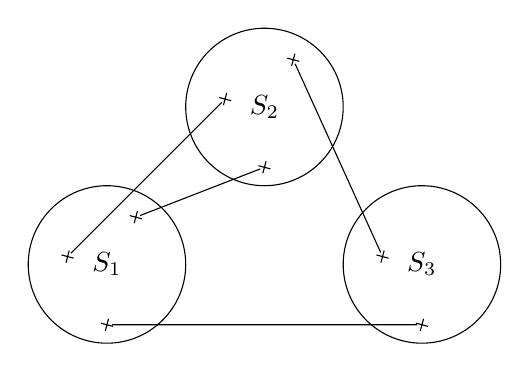
\begin{tikzpicture}
\node (a) [cross,rotate=30] {};
\node (b) [cross,rotate=30,below of = a] {};
\node (c) [cross,rotate=30,right of = a] {};

\node (s1) at (.5,-.1) [draw,circle,minimum size=2cm] {$S_1$};

\node (a1) at (2,2) [cross,rotate=30] {};
\node (b1) [cross,rotate=30,below of = a1] {};
\node (c1) [cross,rotate=30,right of = a1] {};

\node (s2) at (2.5,1.9) [draw,circle,minimum size=2cm] {$S_2$};

\node (a2) at (4,0) [cross,rotate=30] {};
\node (b2) [cross,rotate=30,below of = a2] {};

\node (s3) at (4.5,-.1) [draw,circle,minimum size=2cm] {$S_3$};

\path
(a) edge (a1)
(c) edge (b1)
(c1) edge (a2)
(b) edge (b2)
;
\end{tikzpicture}